\documentclass[11pt,a4paper,oldfontcommands,oneside]{memoir}
\usepackage[utf8]{inputenc}
\usepackage{microtype}
\usepackage[dvips]{graphicx}
\usepackage{xcolor}
\usepackage{times}
\usepackage{graphicx}
\usepackage[spanish]{babel}
\usepackage[
breaklinks=true,colorlinks=true,
%linkcolor=blue,urlcolor=blue,citecolor=blue,% PDF VIEW
linkcolor=black,urlcolor=black,citecolor=black,% PRINT
bookmarks=true,bookmarksopenlevel=2]{hyperref}
\usepackage{pdfpages}
\usepackage{hyperref}
\usepackage{geometry}
% PDF VIEW
% \geometry{total={210mm,297mm},
% left=25mm,right=25mm,%
% bindingoffset=0mm, top=25mm,bottom=25mm}
% PRINT
\geometry{total={210mm,297mm},
left=20mm,right=20mm,
bindingoffset=10mm, top=25mm,bottom=25mm}

\OnehalfSpacing
%\linespread{1.3}

%%% CHAPTER'S STYLE
\chapterstyle{bianchi}
%\chapterstyle{ger}
%\chapterstyle{madsen}
%\chapterstyle{ell}
%%% STYLE OF SECTIONS, SUBSECTIONS, AND SUBSUBSECTIONS
\setsecheadstyle{\Large\bfseries\sffamily\raggedright}
\setsubsecheadstyle{\large\bfseries\sffamily\raggedright}
\setsubsubsecheadstyle{\bfseries\sffamily\raggedright}


%%% STYLE OF PAGES NUMBERING
%\pagestyle{companion}\nouppercaseheads 
%\pagestyle{headings}
%\pagestyle{Ruled}
\pagestyle{plain}
\makepagestyle{plain}
\makeevenfoot{plain}{\thepage}{}{}
\makeoddfoot{plain}{}{}{\thepage}
\makeevenhead{plain}{}{}{}
\makeoddhead{plain}{}{}{}


\maxsecnumdepth{subsection} % chapters, sections, and subsections are numbered
\maxtocdepth{subsection} % chapters, sections, and subsections are in the Table of Contents


%%%---%%%---%%%---%%%---%%%---%%%---%%%---%%%---%%%---%%%---%%%---%%%---%%%

\begin{document}

%%%---%%%---%%%---%%%---%%%---%%%---%%%---%%%---%%%---%%%---%%%---%%%---%%%
%   TITLEPAGE
%
%   due to variety of titlepage schemes it is probably better to make titlepage manually
%
%%%---%%%---%%%---%%%---%%%---%%%---%%%---%%%---%%%---%%%---%%%---%%%---%%%
\thispagestyle{empty}

{%%%
\sffamily
\centering
\Large

~\vspace{\fill}

\includegraphics[scale=1]{Escudo.png} \\
{\huge 
\vspace{4cm}
Brazo Robótico Pintador Tipo Esférico 
}
\vspace{2.5cm}

{\LARGE
Cesar Omar Alvarado Contreras\\
Marco Manzo Torrez\\
Eduardo Robles Vázquez\\
Víctor Gabriel Tapia Casillas\\
Fonseca Camarena Jonathan
}

\vspace{2.5cm}

Universidad Politécnica de la Zona Metropolitana de Guadalajara

\vspace{3.5cm}

Proyecto Anual

\vspace{\fill}

8 de Noviembre de 2019

%%%
}%%%

\vspace{.5cm}
\hfill\break




\tableofcontents*

\clearpage

%%%---%%%---%%%---%%%---%%%---%%%---%%%---%%%---%%%---%%%---%%%---%%%---%%%
%%%---%%%---%%%---%%%---%%%---%%%---%%%---%%%---%%%---%%%---%%%---%%%---%%%

\chapter{Introducción}
\section{Meta}
Crear un robot polar de tres grados de libertad, con una longitud total de 50 centímetros y una altura total de 30 centímetros, cuyo último eslabón deberá soportar una carga de 500 gramos y tendrá como fin pintar.

\section{Objetivos:}
\noindent
-Realizar boceto\\
-Cumplir con las especificaciones propuestas por el profesor\\
-Realizar el plano del robot\\
-Realizar el modelado del prototipo en 3D\\
-Establecer los materiales a usar\\ 
-Realizar el análisis de elementos finitos\\
-Realizar cálculos necesarios para la selección de motores y componentes\\
-Elaboración del primer prototipo\\
-Programación del robot\\

\section{Justificación}
El propósito de este proyecto surge a partir de la necesidad de implementar los conocimientos obtenidos de las materias presentes de estos ultimos 3 cuatrimestres, así como de cuatrimestres pasados.
Retomando lo mencionado con anterioridad, se desarrollará un prototipo de un brazo robótico polar, el cual consistirá de 3 grados de libertad; dos movimientos rotacionales y uno prismático.

\chapter{Desarrollo}
\section{Tabla de materias}
A continuación, presentamos la tabla de materias que nos ayudarán en nuestro proyecto.\\
\begin{center}
\includegraphics[width=15cm]{tabla.png}
 \\
 Figura 1: Tabla 
\end{center}



\section{Project}
En el programa Project realizamos el cronograma de actividades.\\

\begin{center}
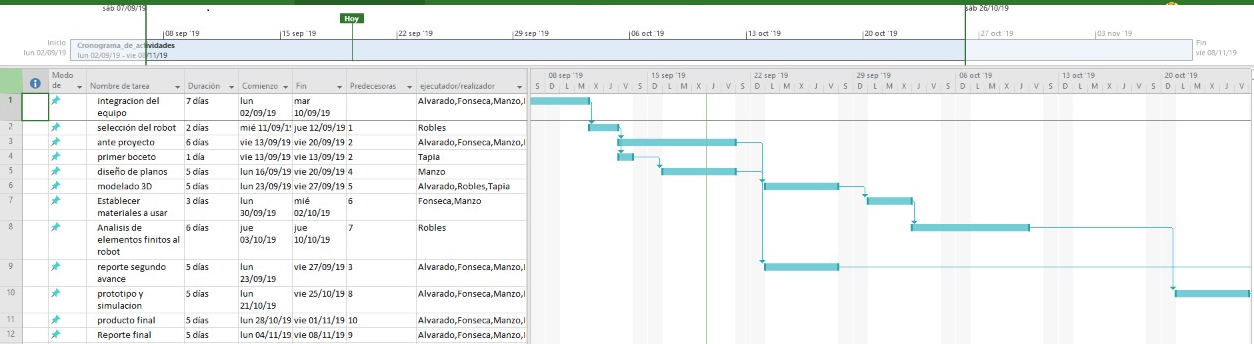
\includegraphics[width=18cm]{Project.png}
   Figura 2: Project
    
\end{center}



\section{Proposición del análisis finito}
Lo que se pretende calcular del robot, es la cantidad que puede soportar, esperando como resultado una carga de 500 gramos, calcular los diámetros correspondientes a los pasadores para evitar cargas por cortante; selección del material para la estructura y actuadores, como también el cálculo de estimación del tiempo de vida del robot.\\

\section{Material seleccionado}

Para darle una mayor resistencia a la estructura del robot se planea utilizar una aleación de aluminio, ya que tiene mayor resistencia al desgaste y deformación a diferencia de otros materiales además de ser relativamente ligero.\\


\begin{center}
\includegraphics[width=10cm]{tablaaluminio.png}
 \\
 Figura 3: Tabla Aluminio
\end{center}
Posteriormente se realizará una prueba de elementos finitos mediante un software para sustentar la idea de dicho material.\\

\section{Cronograma de gastos de elaboración de robot esférico}
 
\begin{center}
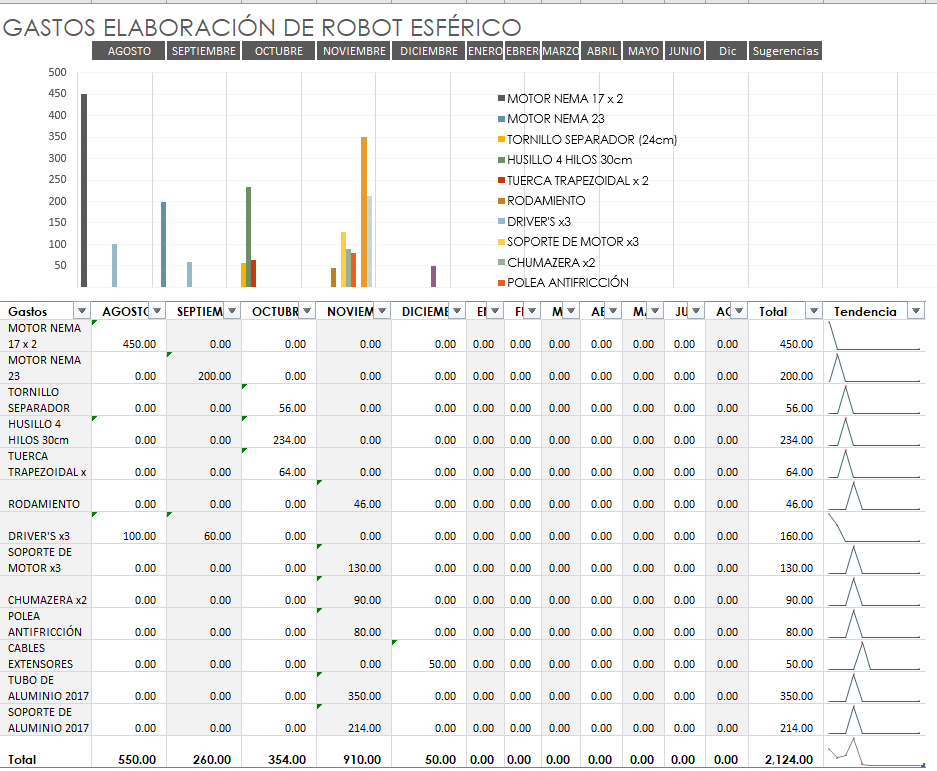
\includegraphics[width=16cm]{2019-10-18.png}
 Figura4 :Gastos de elaboración
\end{center}
    
\section{Avances relacionados con las materias}
\subsection{Diseño y selección de elementos mecánicos}
El avance que se ha obtenido en esta materia ha sido en cuanto al diseño de las piezas y el ensamble del modelado 3D en el software Inventor, además del análisis de elementos finitos, el cúal, brindó una clara observación de los materiales que serán mas convenientes de usar para no sufrir alguna deformación o daño de la estructura.\\

\begin{center}
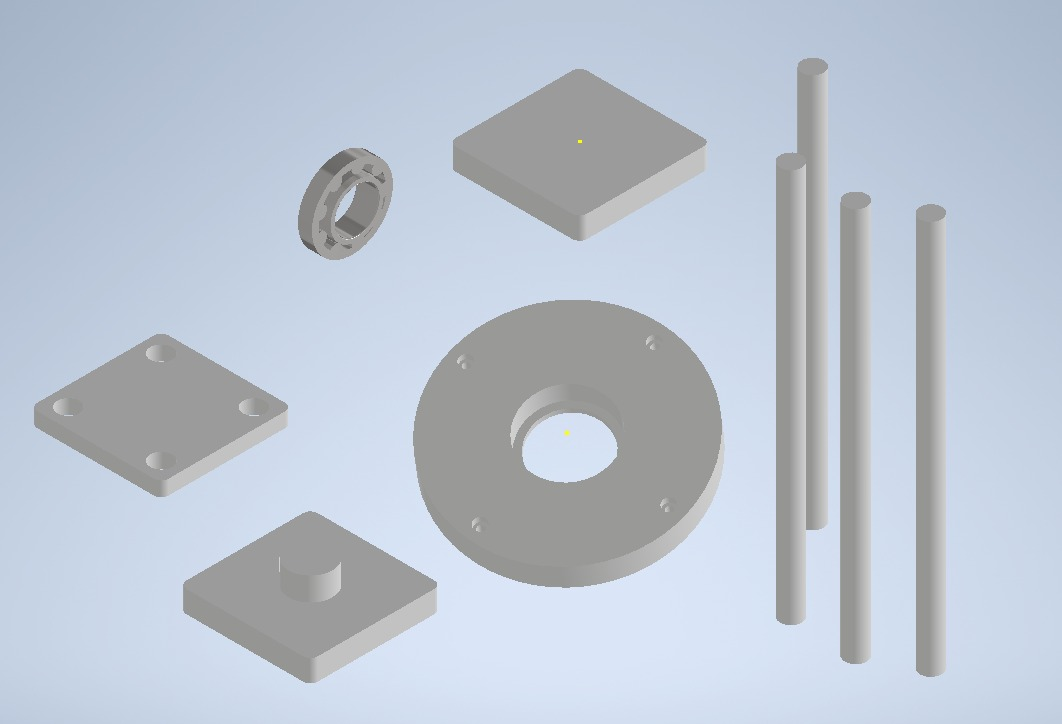
\includegraphics[width=5cm]{Dibujo1.jpeg}
 \\
 Figura 5:Dibujo1
\end{center}

Fue necesario realizar los dibujos varias ocasiones por que encontraba algún problema ya sea de medida o de fricción en las piezas de nuestro proyecto.\\
\begin{center}
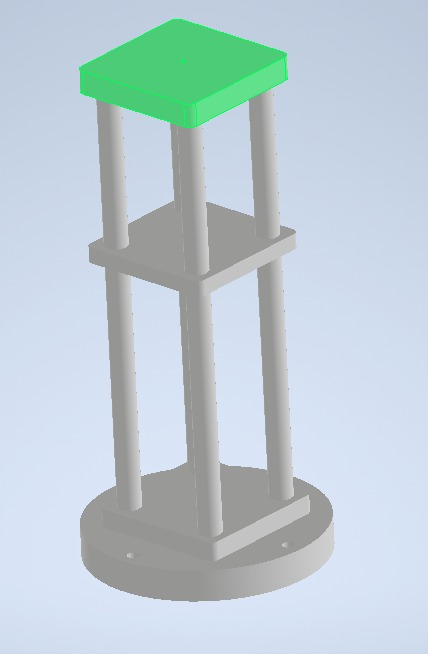
\includegraphics[width=5cm]{Dibujo2.jpeg}
 \\
 Figura 6:Dibujo2
\end{center}

Asimismo, entendimos cómo convertir una idea de diseño en un producto real, eligiendo la mejor opción en cuanto al enfoque, las técnicas y los materiales a utilizar. Nuestro proyecto se emplea en el diseño asistido por ordenador (CAD) para llevar a término este proyecto.

\subsection{Modelado y simulación de sistemas}
La propuesta de modelado matemático que se desarrollará será un modelo dinámico en el robot de forma sistemática, logrando expresar todos los fenómenos físicos presentes en el movimiento del mecanismo a través de las ecuaciones de movimiento de Euler-Lagrange.

\subsection{Cinemática de robots}
Se ha realizado el modelo cinemático directo del robot obtenido por medio de la metodología Denavit-Hartenberg y las transformaciones homogéneas, lo cual describe la posición en el espacio del mismo.

\section{Simulación de cinemática directa e inversa}
En esta práctica se describió el funcionamiento del robot mediante modelados matemáticos que permiten describir los movimientos y parámetros de los ejes del robot.\\
A continuación se anexarán páginas referentes a este apartado:

\includepdf[pages=4-5]{simulacion}

\section{Análisis de elementos finitos}
Como se demostró previamente en una práctica, se hizo una comparación entre distintos materiales, de los cuales, finalmente se optó por la madera, debido a sus propiedades, ésta resiste sin problema alguno el peso de la estructura y a la vez el peso del objeto a sostener que es de 500 gramos.\\
A continuación se anexarán páginas referentes a este apartado:

\includepdf[pages=6]{elementos}
\includepdf[pages=16]{elementos}
\includepdf[pages=8]{elementos}
\includepdf[pages=20]{elementos}

\chapter{Fotografías del armado de prototipo}
A continuación se mostrararán imágenes del armado y desarrollo del prototipo.
\begin{center}
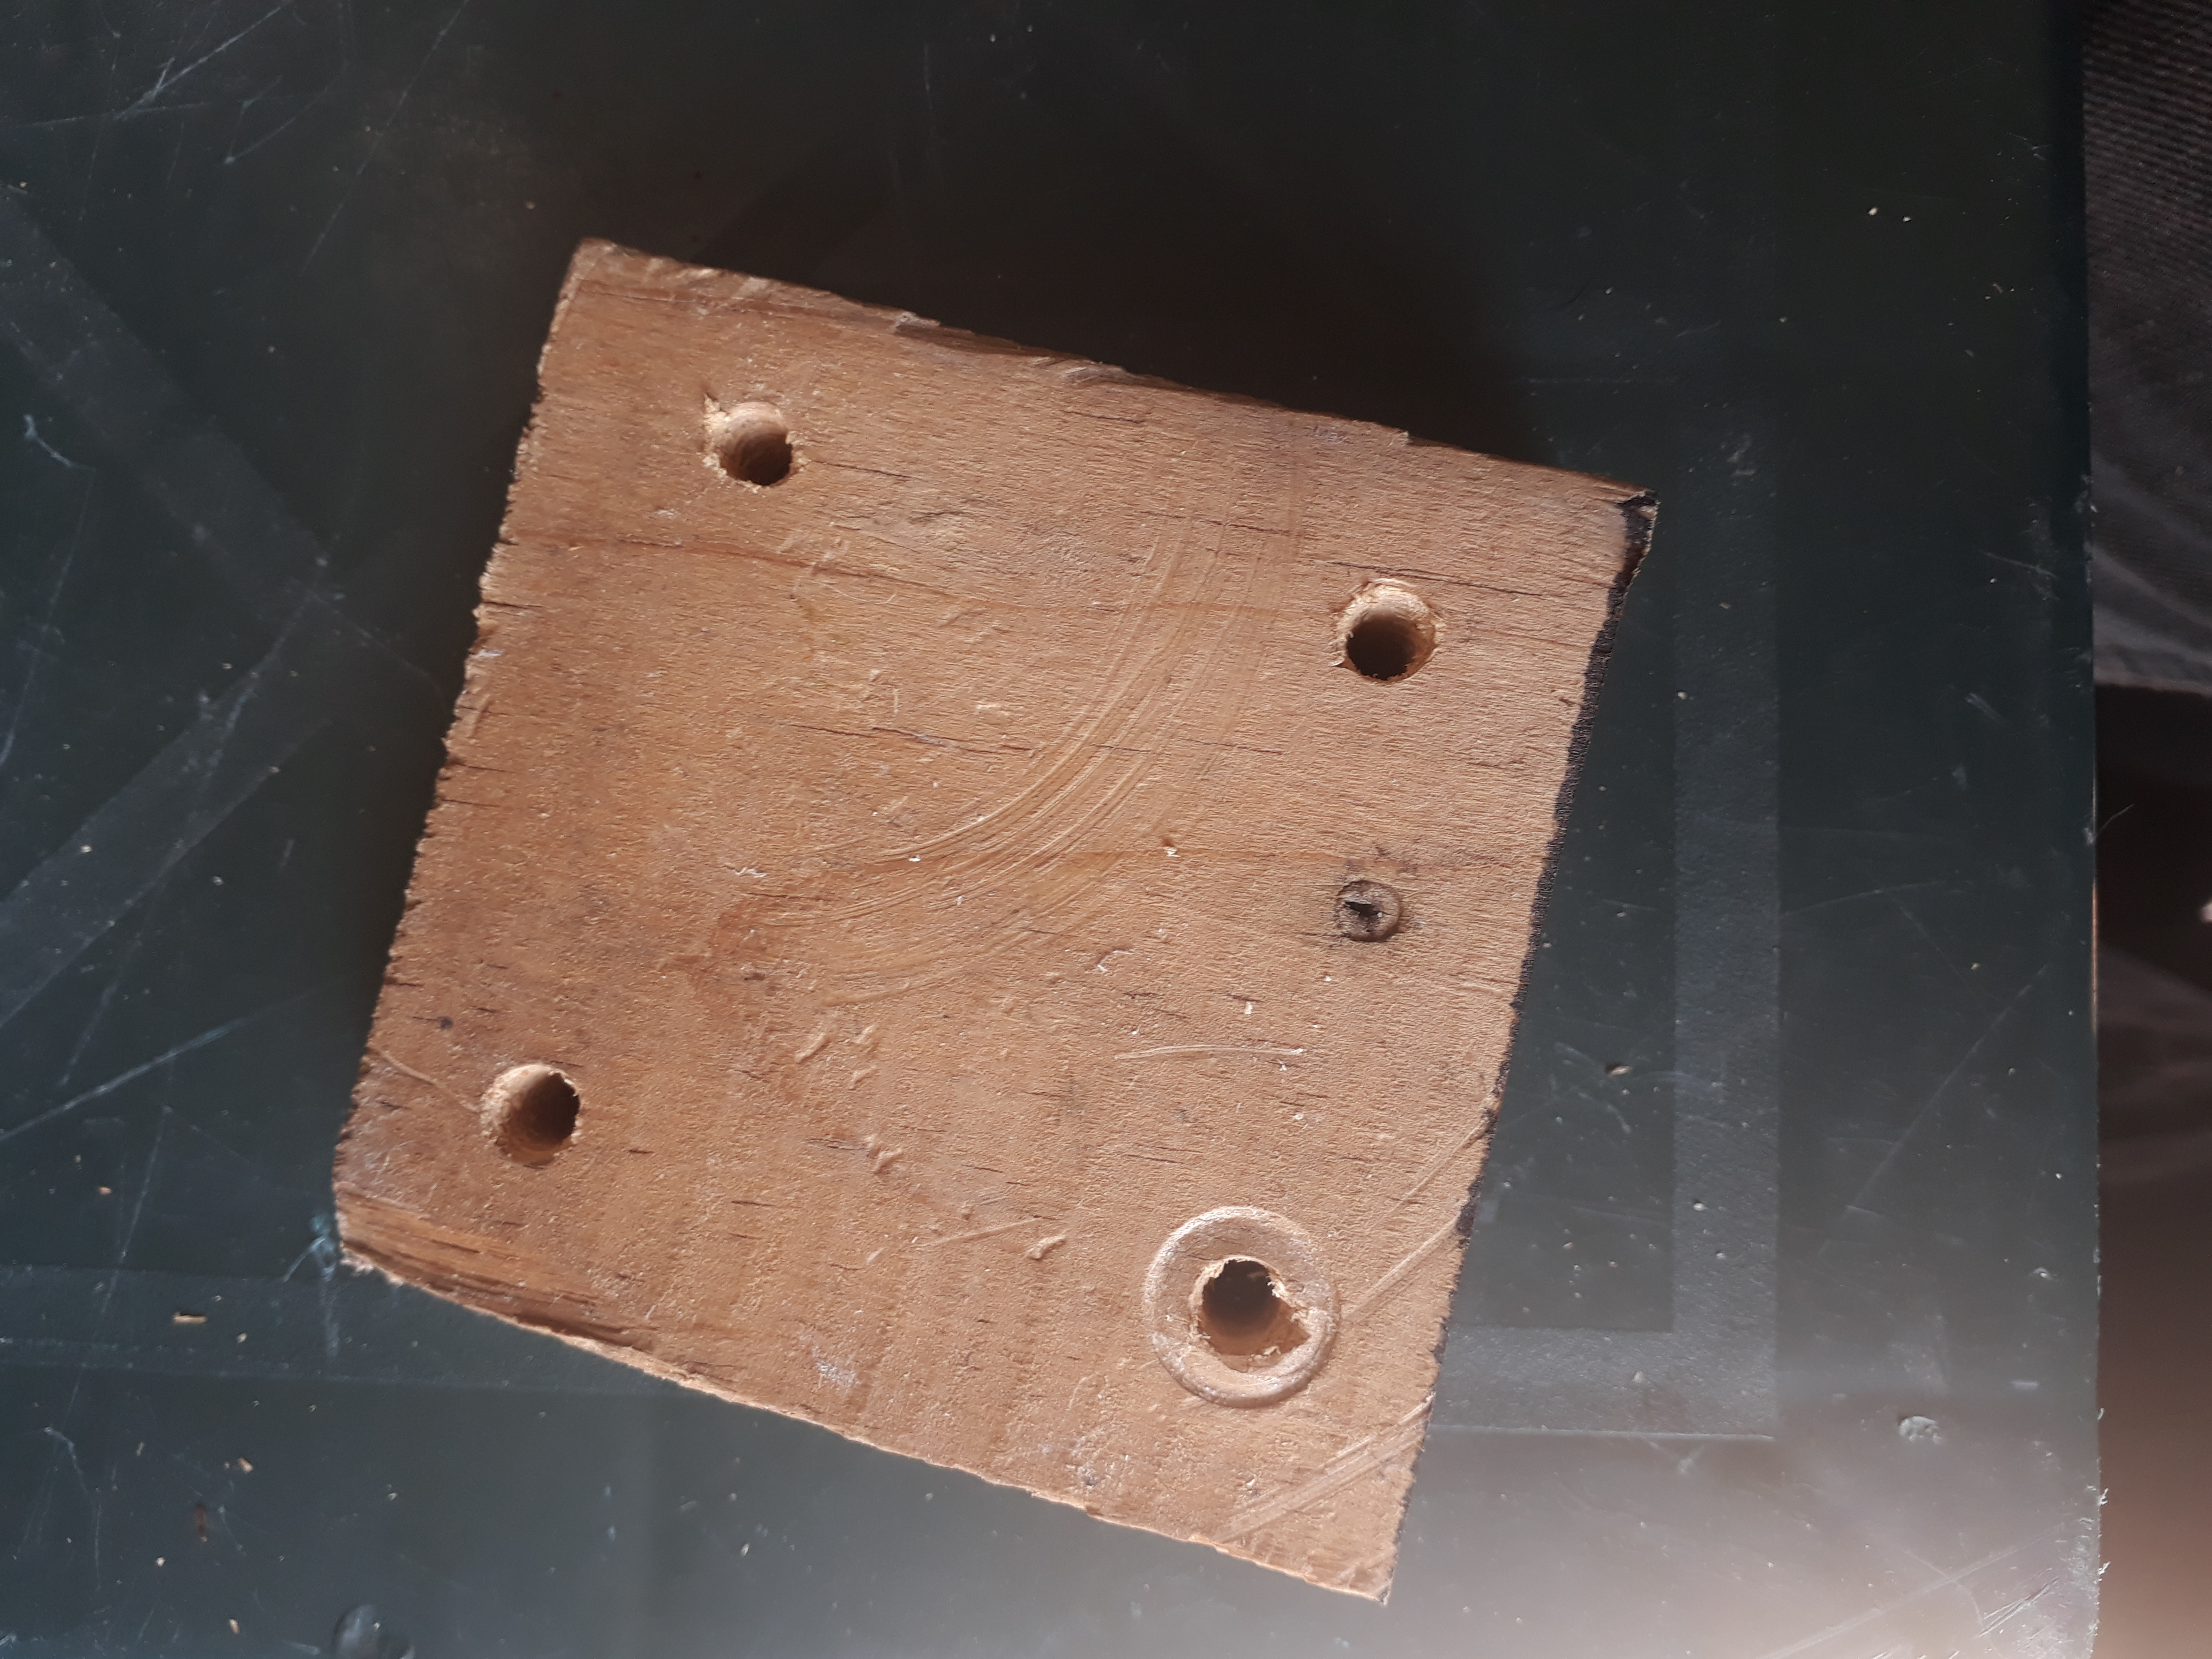
\includegraphics[scale=0.05]{1.jpg} \\
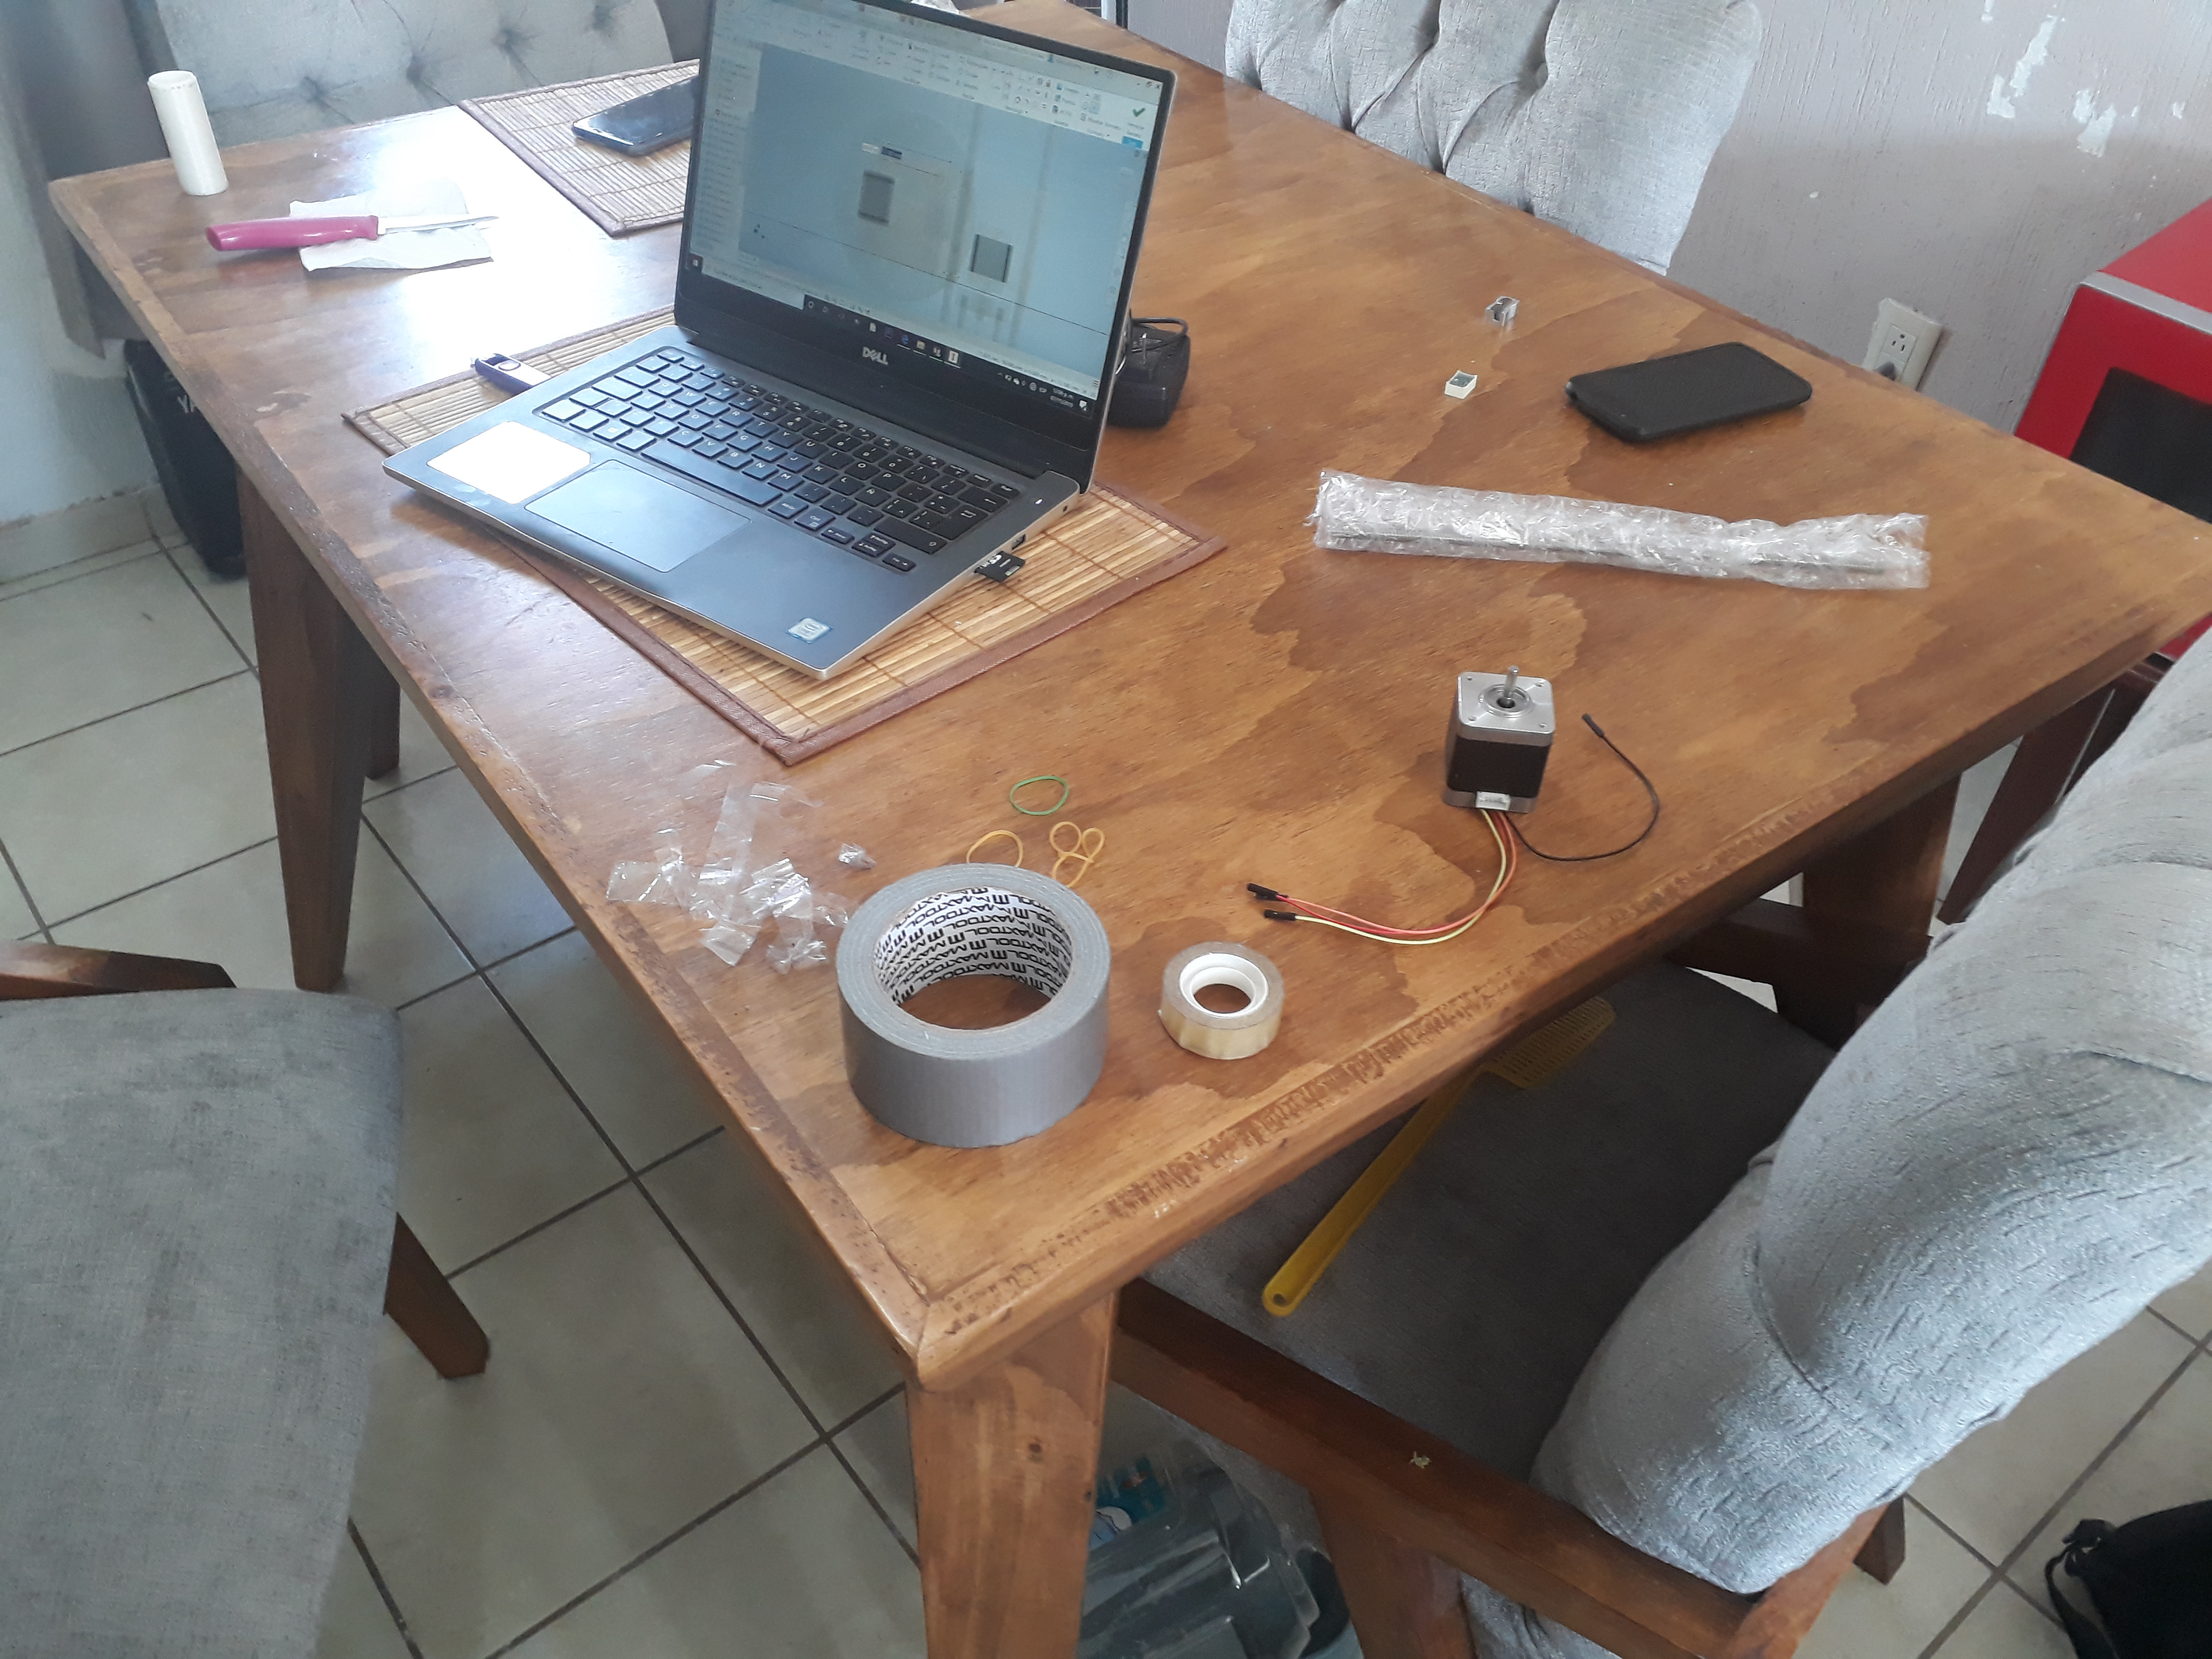
\includegraphics[scale=0.05]{2.jpg} \\
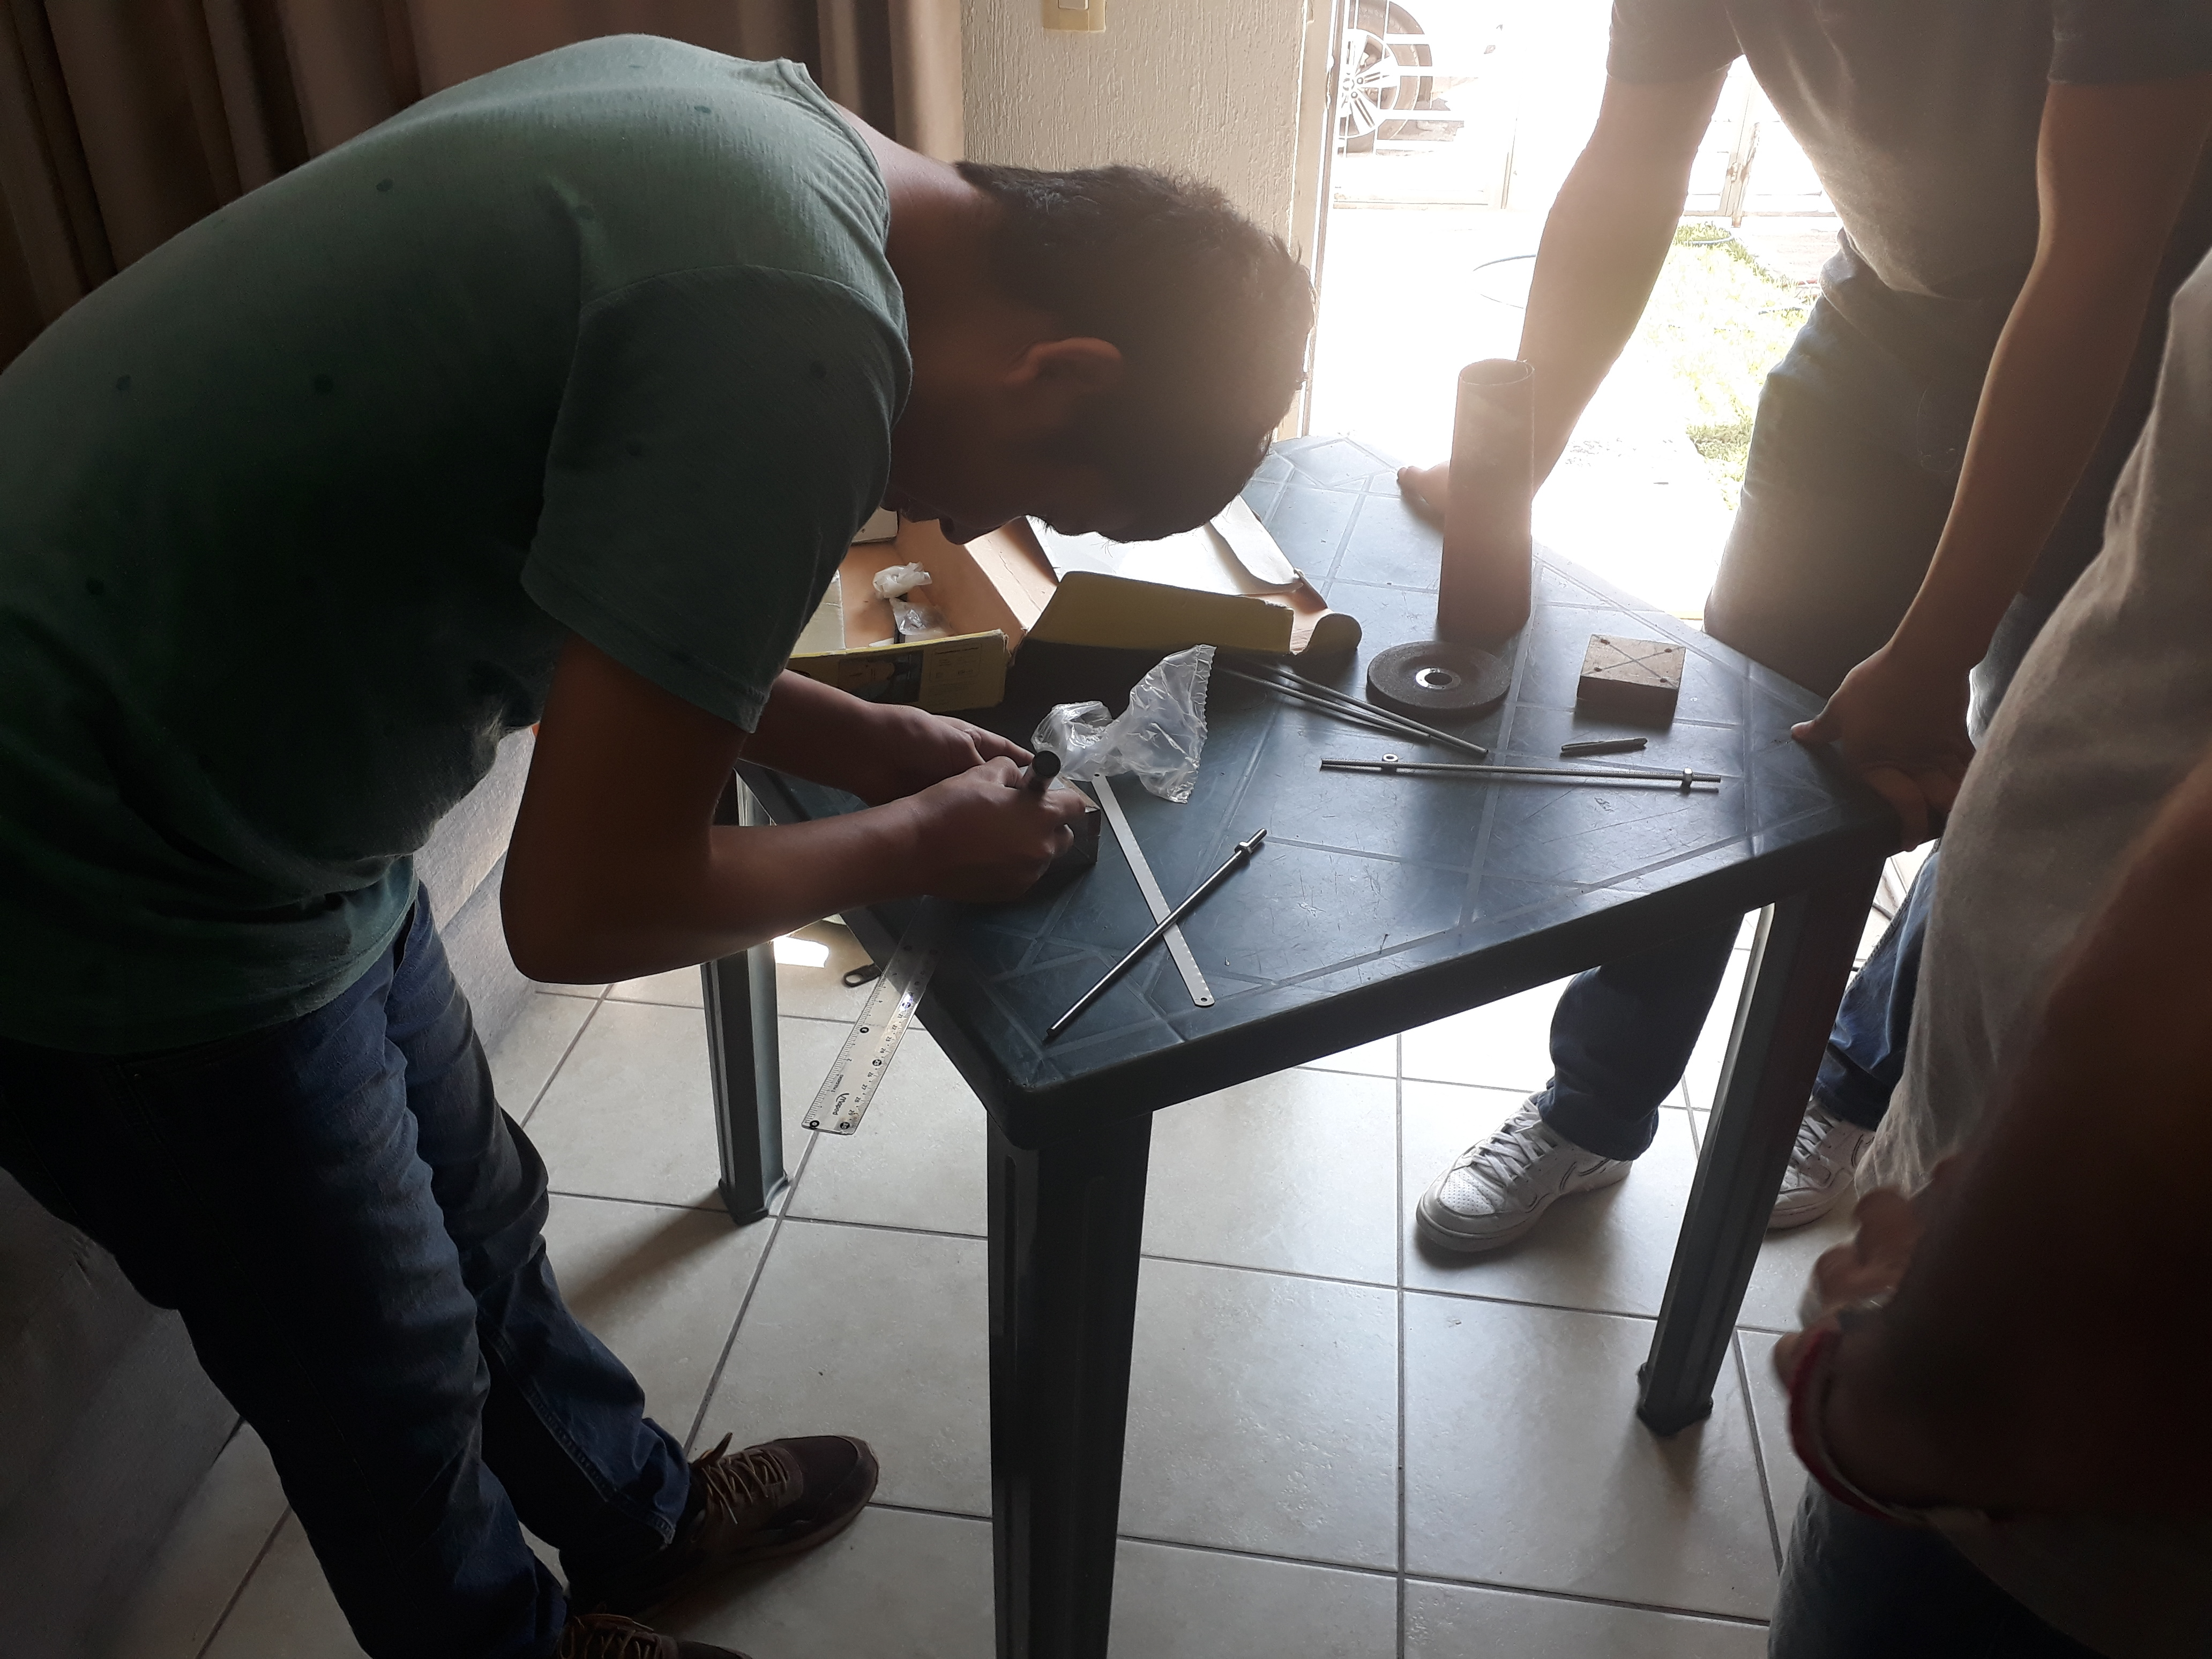
\includegraphics[scale=0.05]{3.jpg} \\
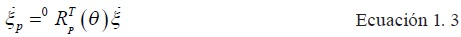
\includegraphics[scale=0.05]{4.jpg} \\
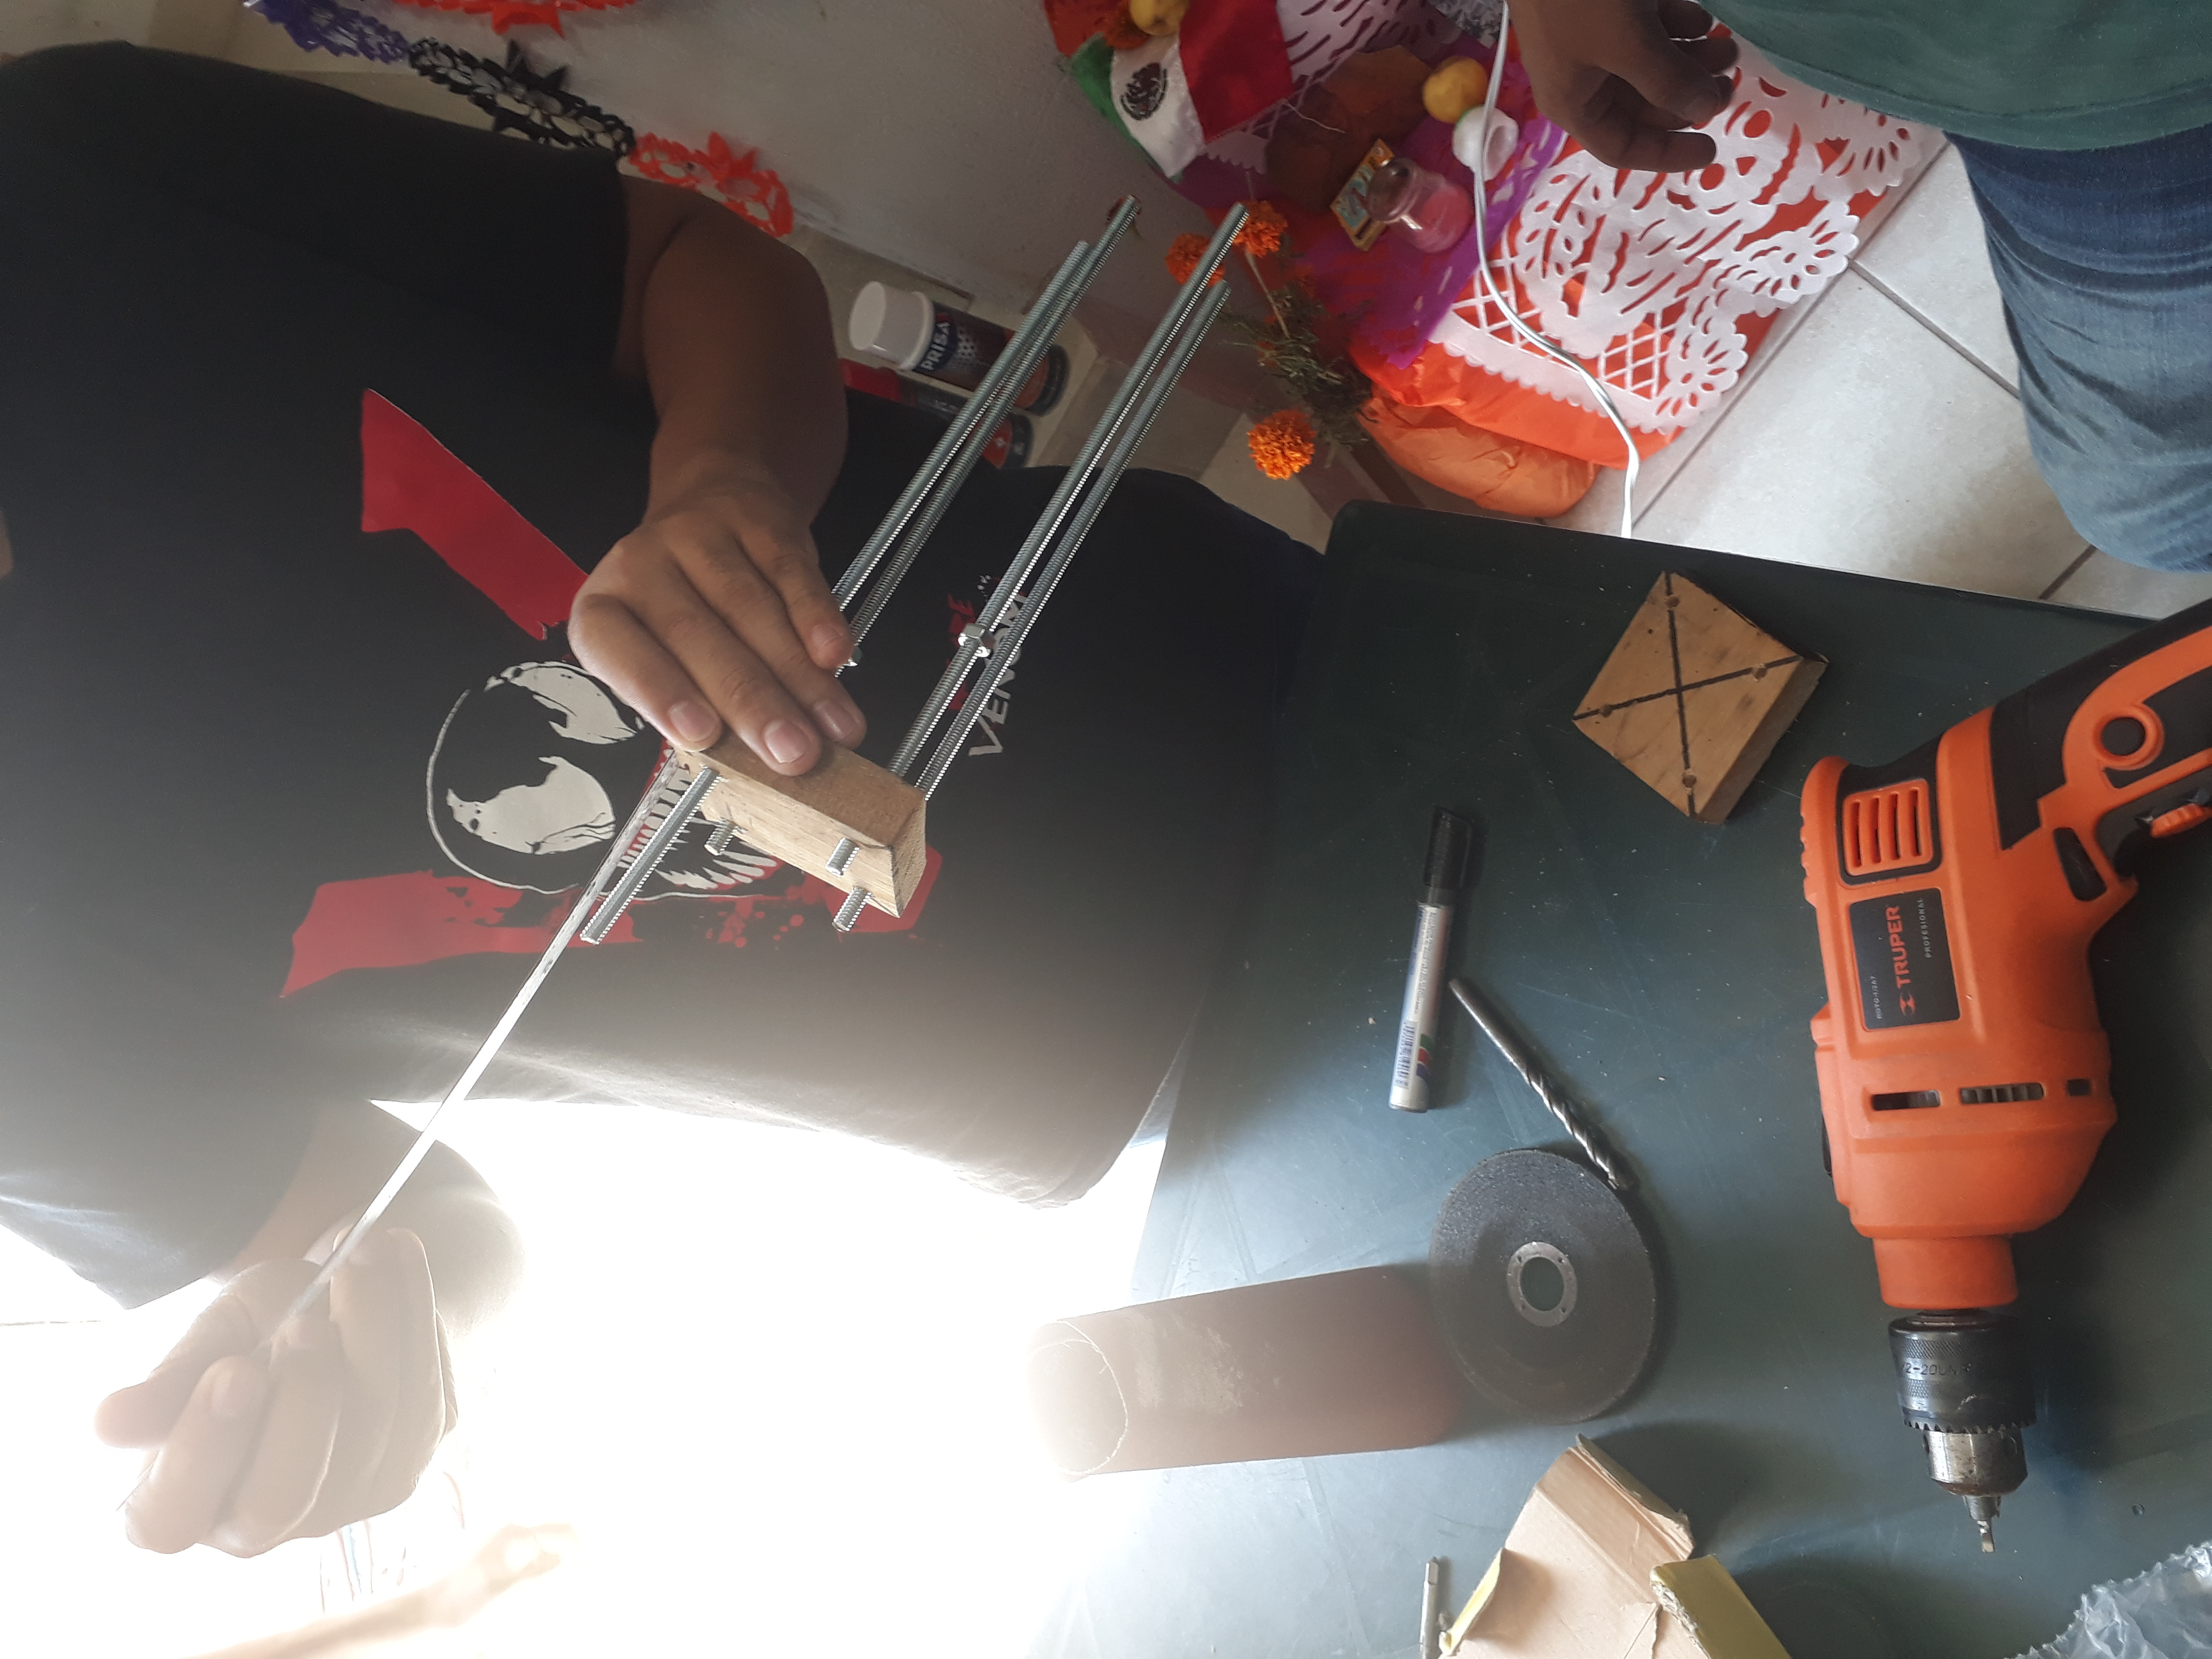
\includegraphics[scale=0.05]{5.jpg} \\
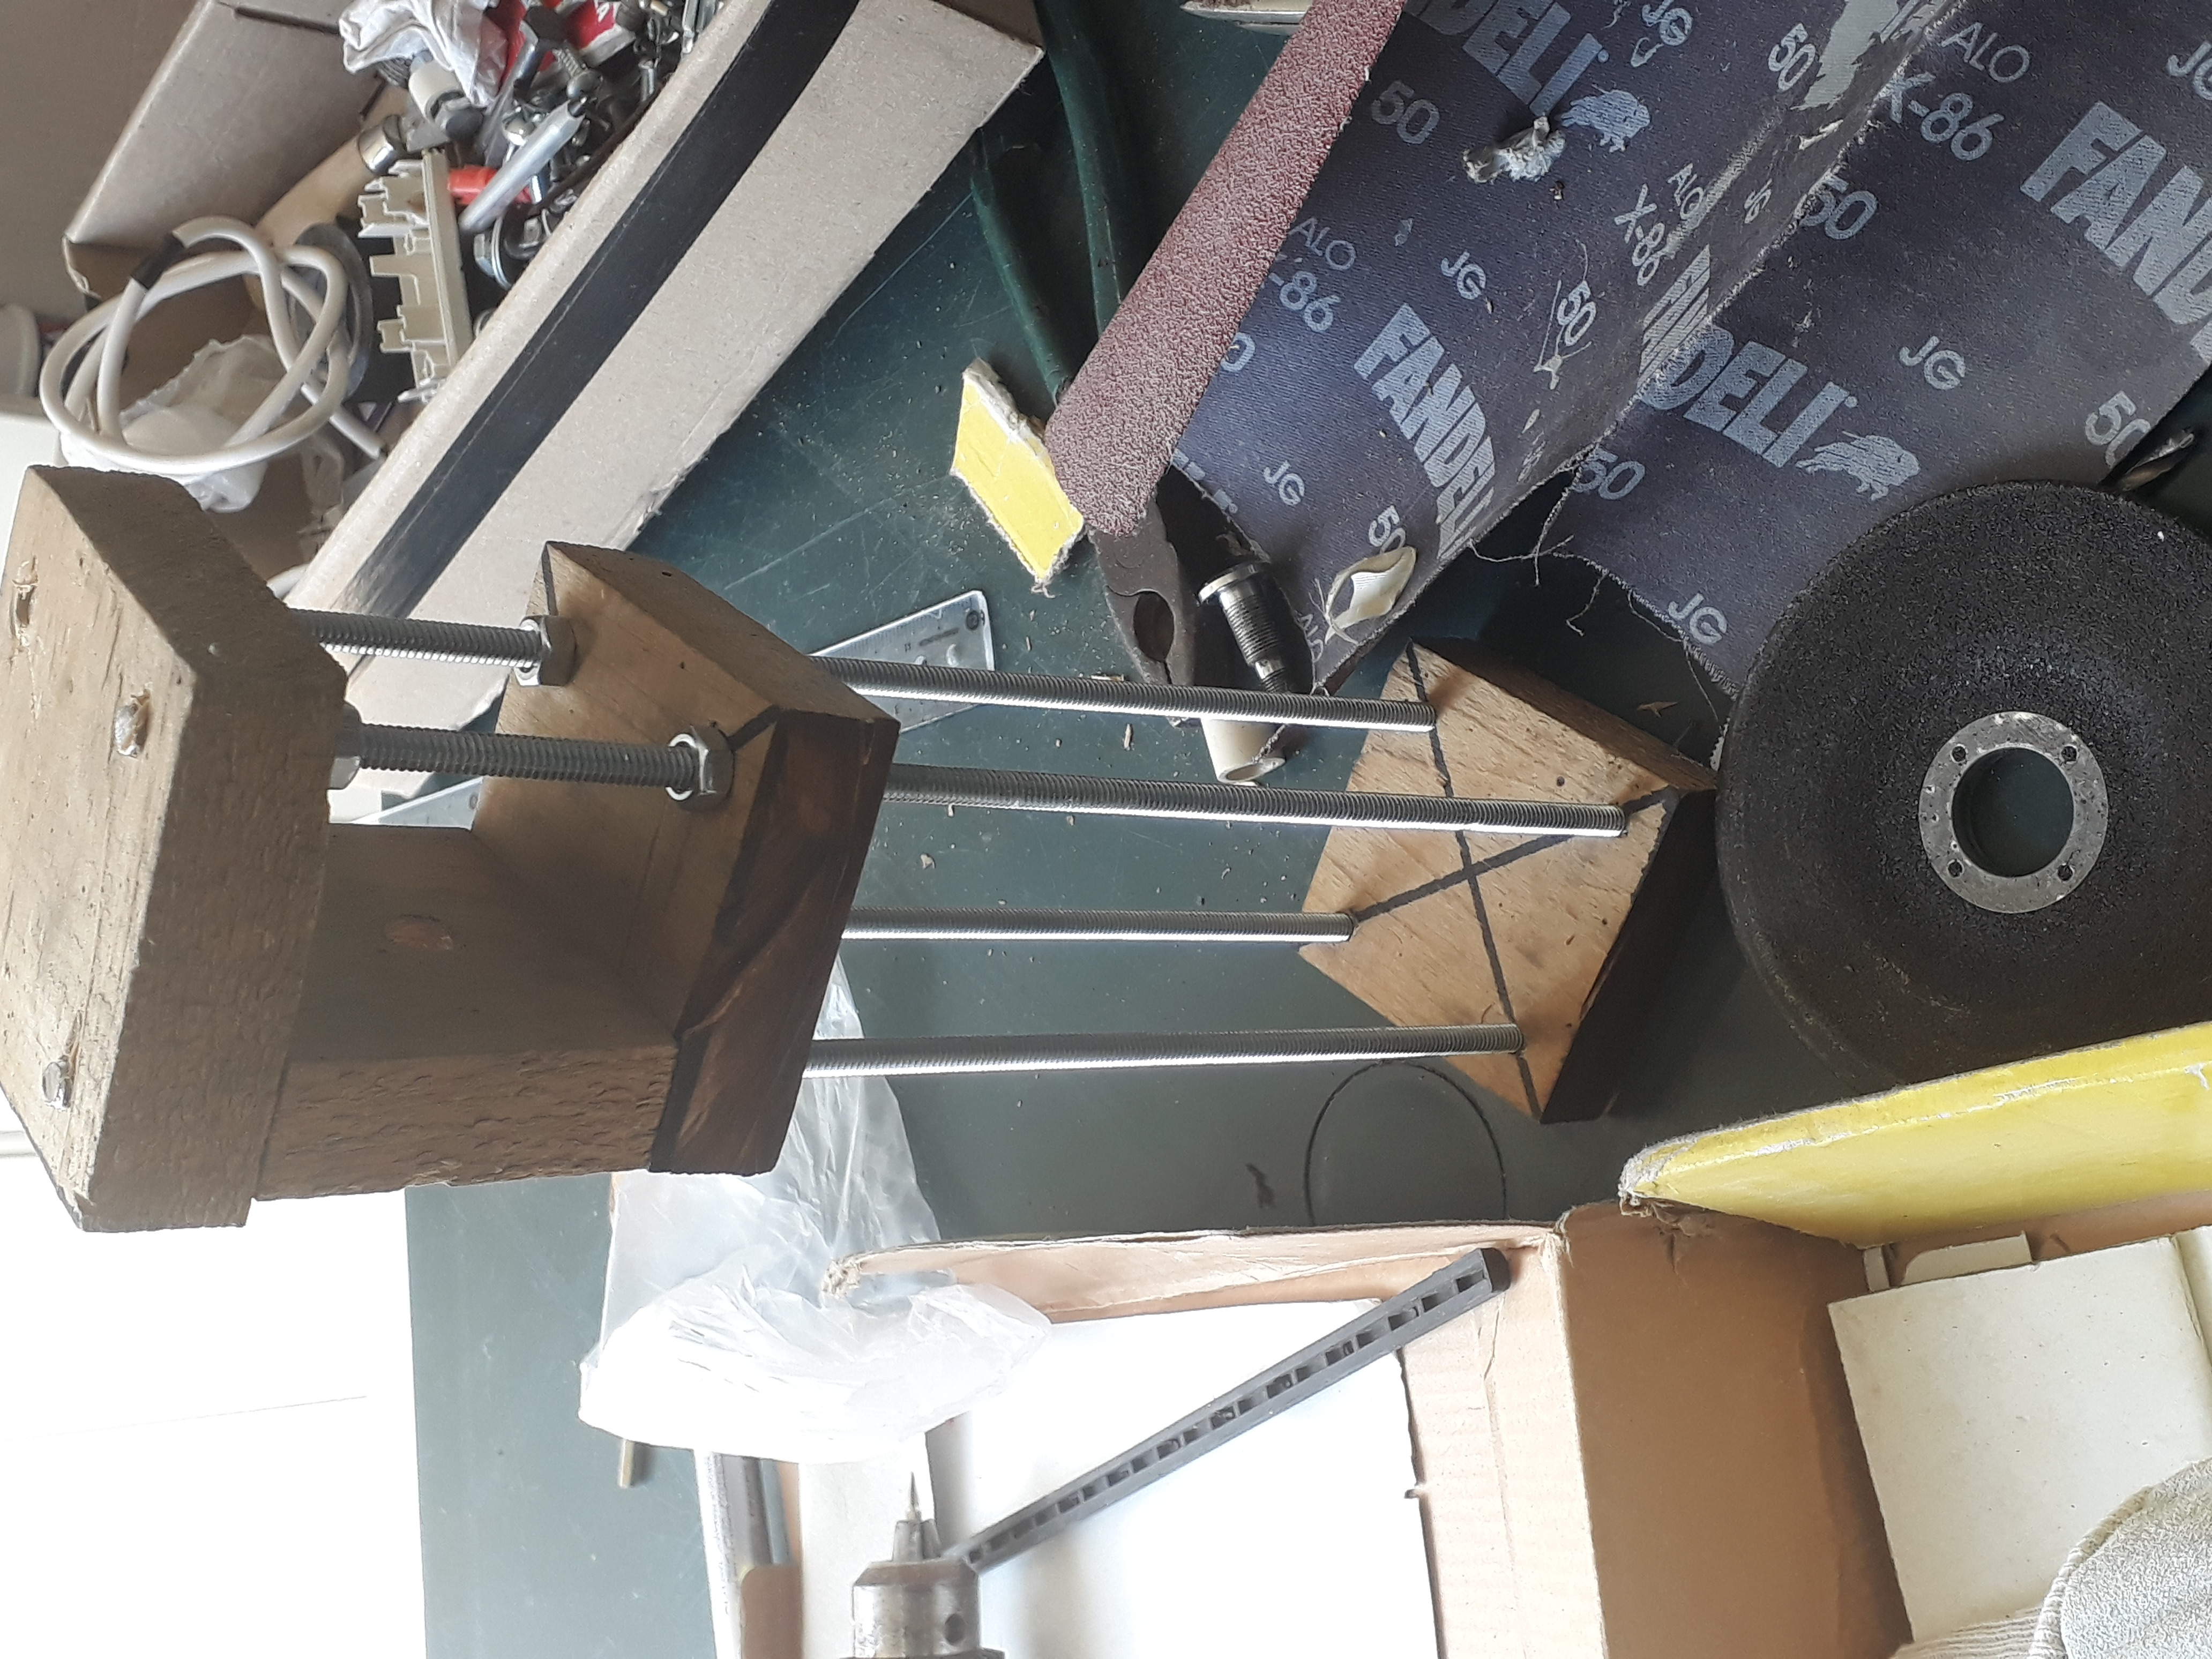
\includegraphics[scale=0.05]{6.jpg} \\
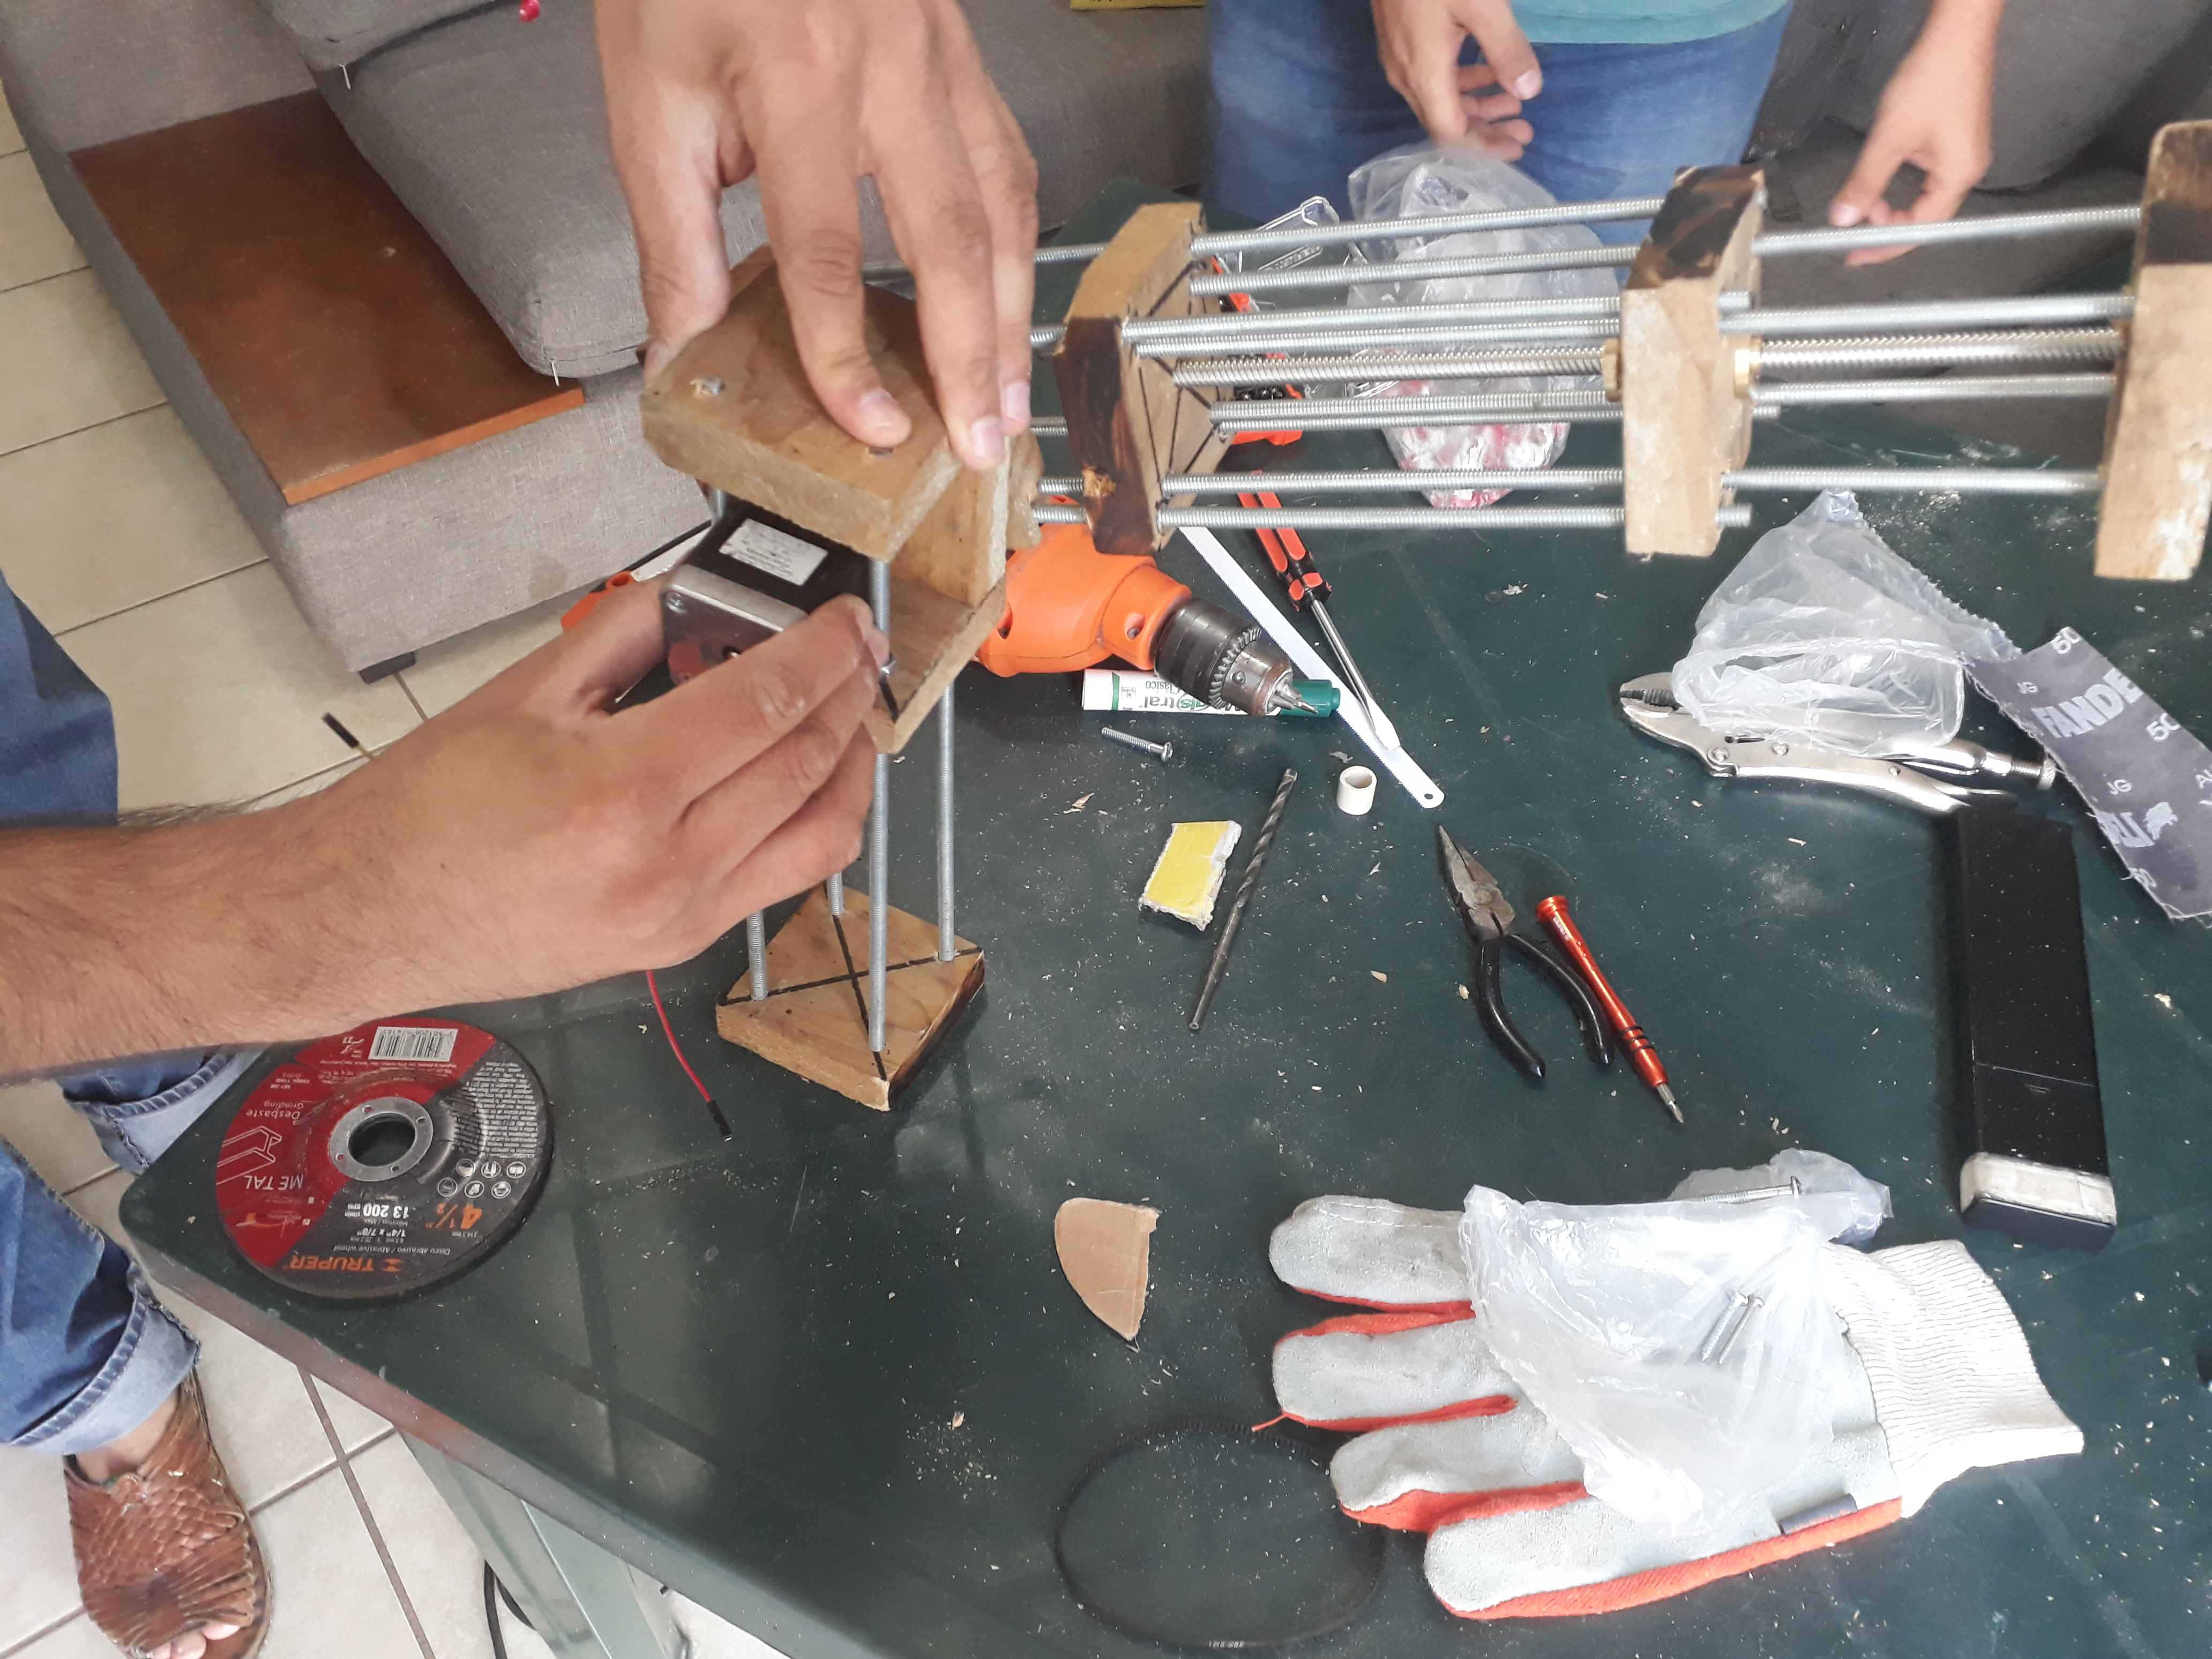
\includegraphics[scale=0.05]{7.jpg} \\
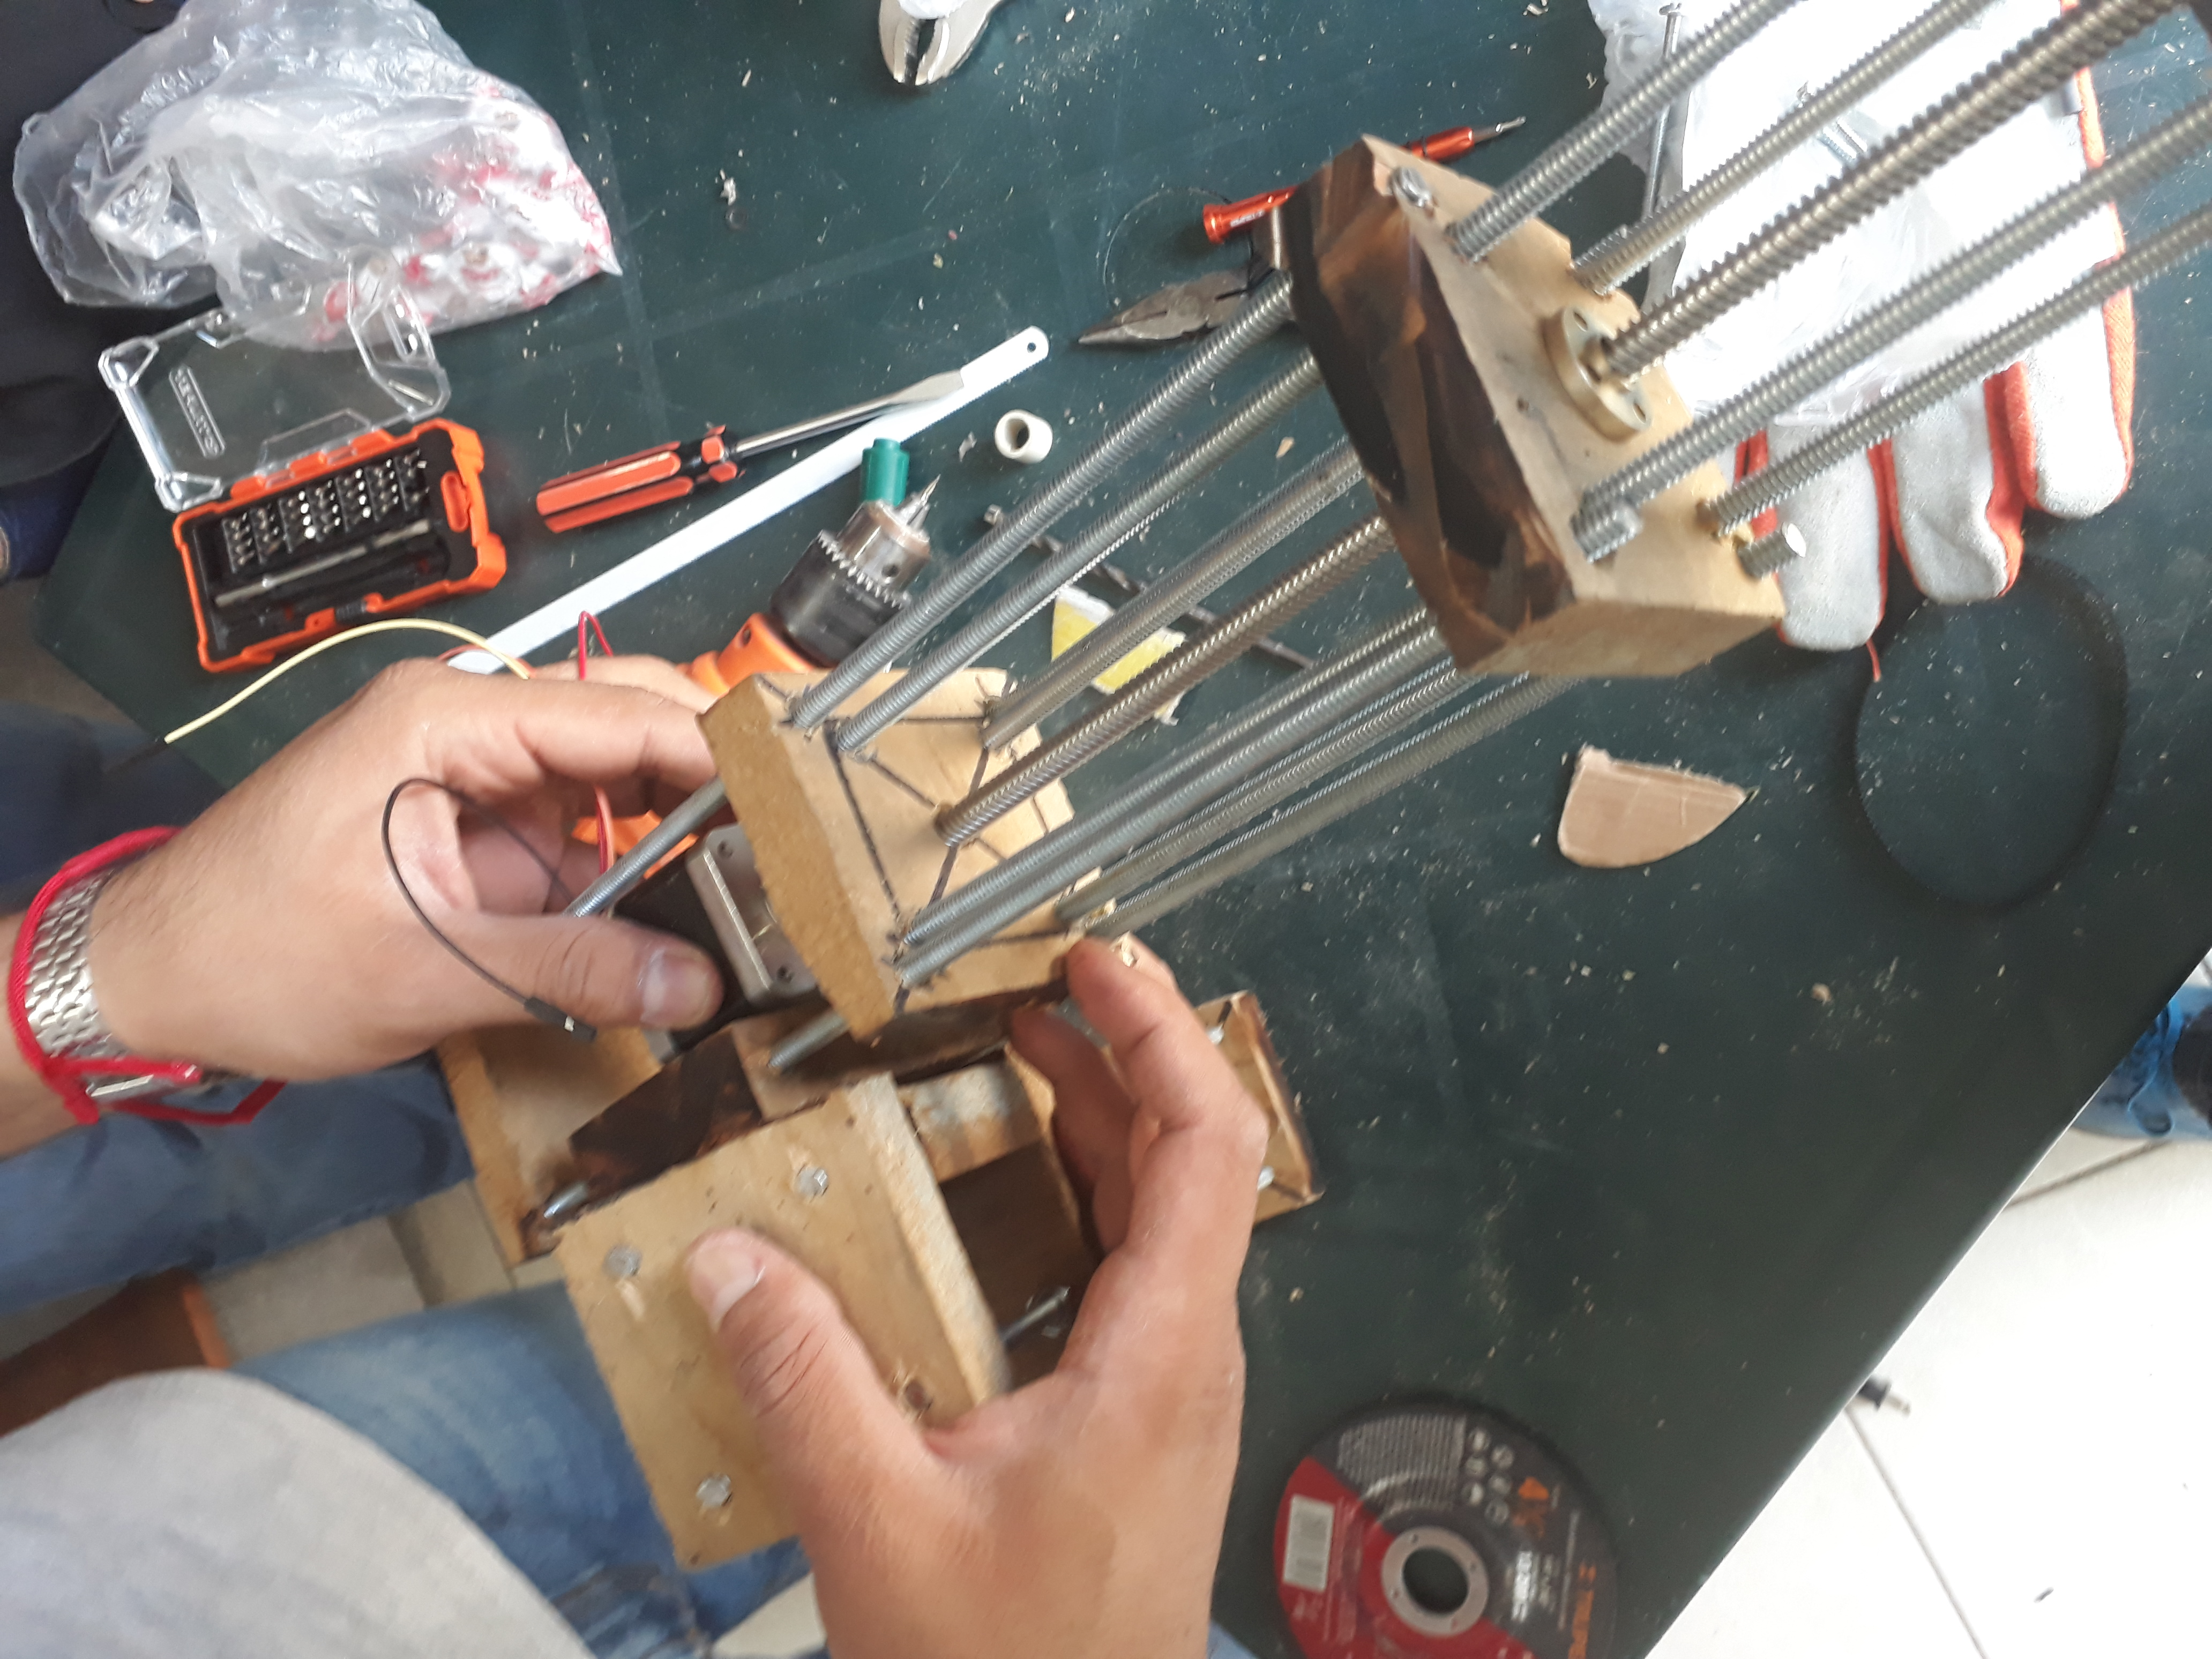
\includegraphics[scale=0.05]{8.jpg} \\
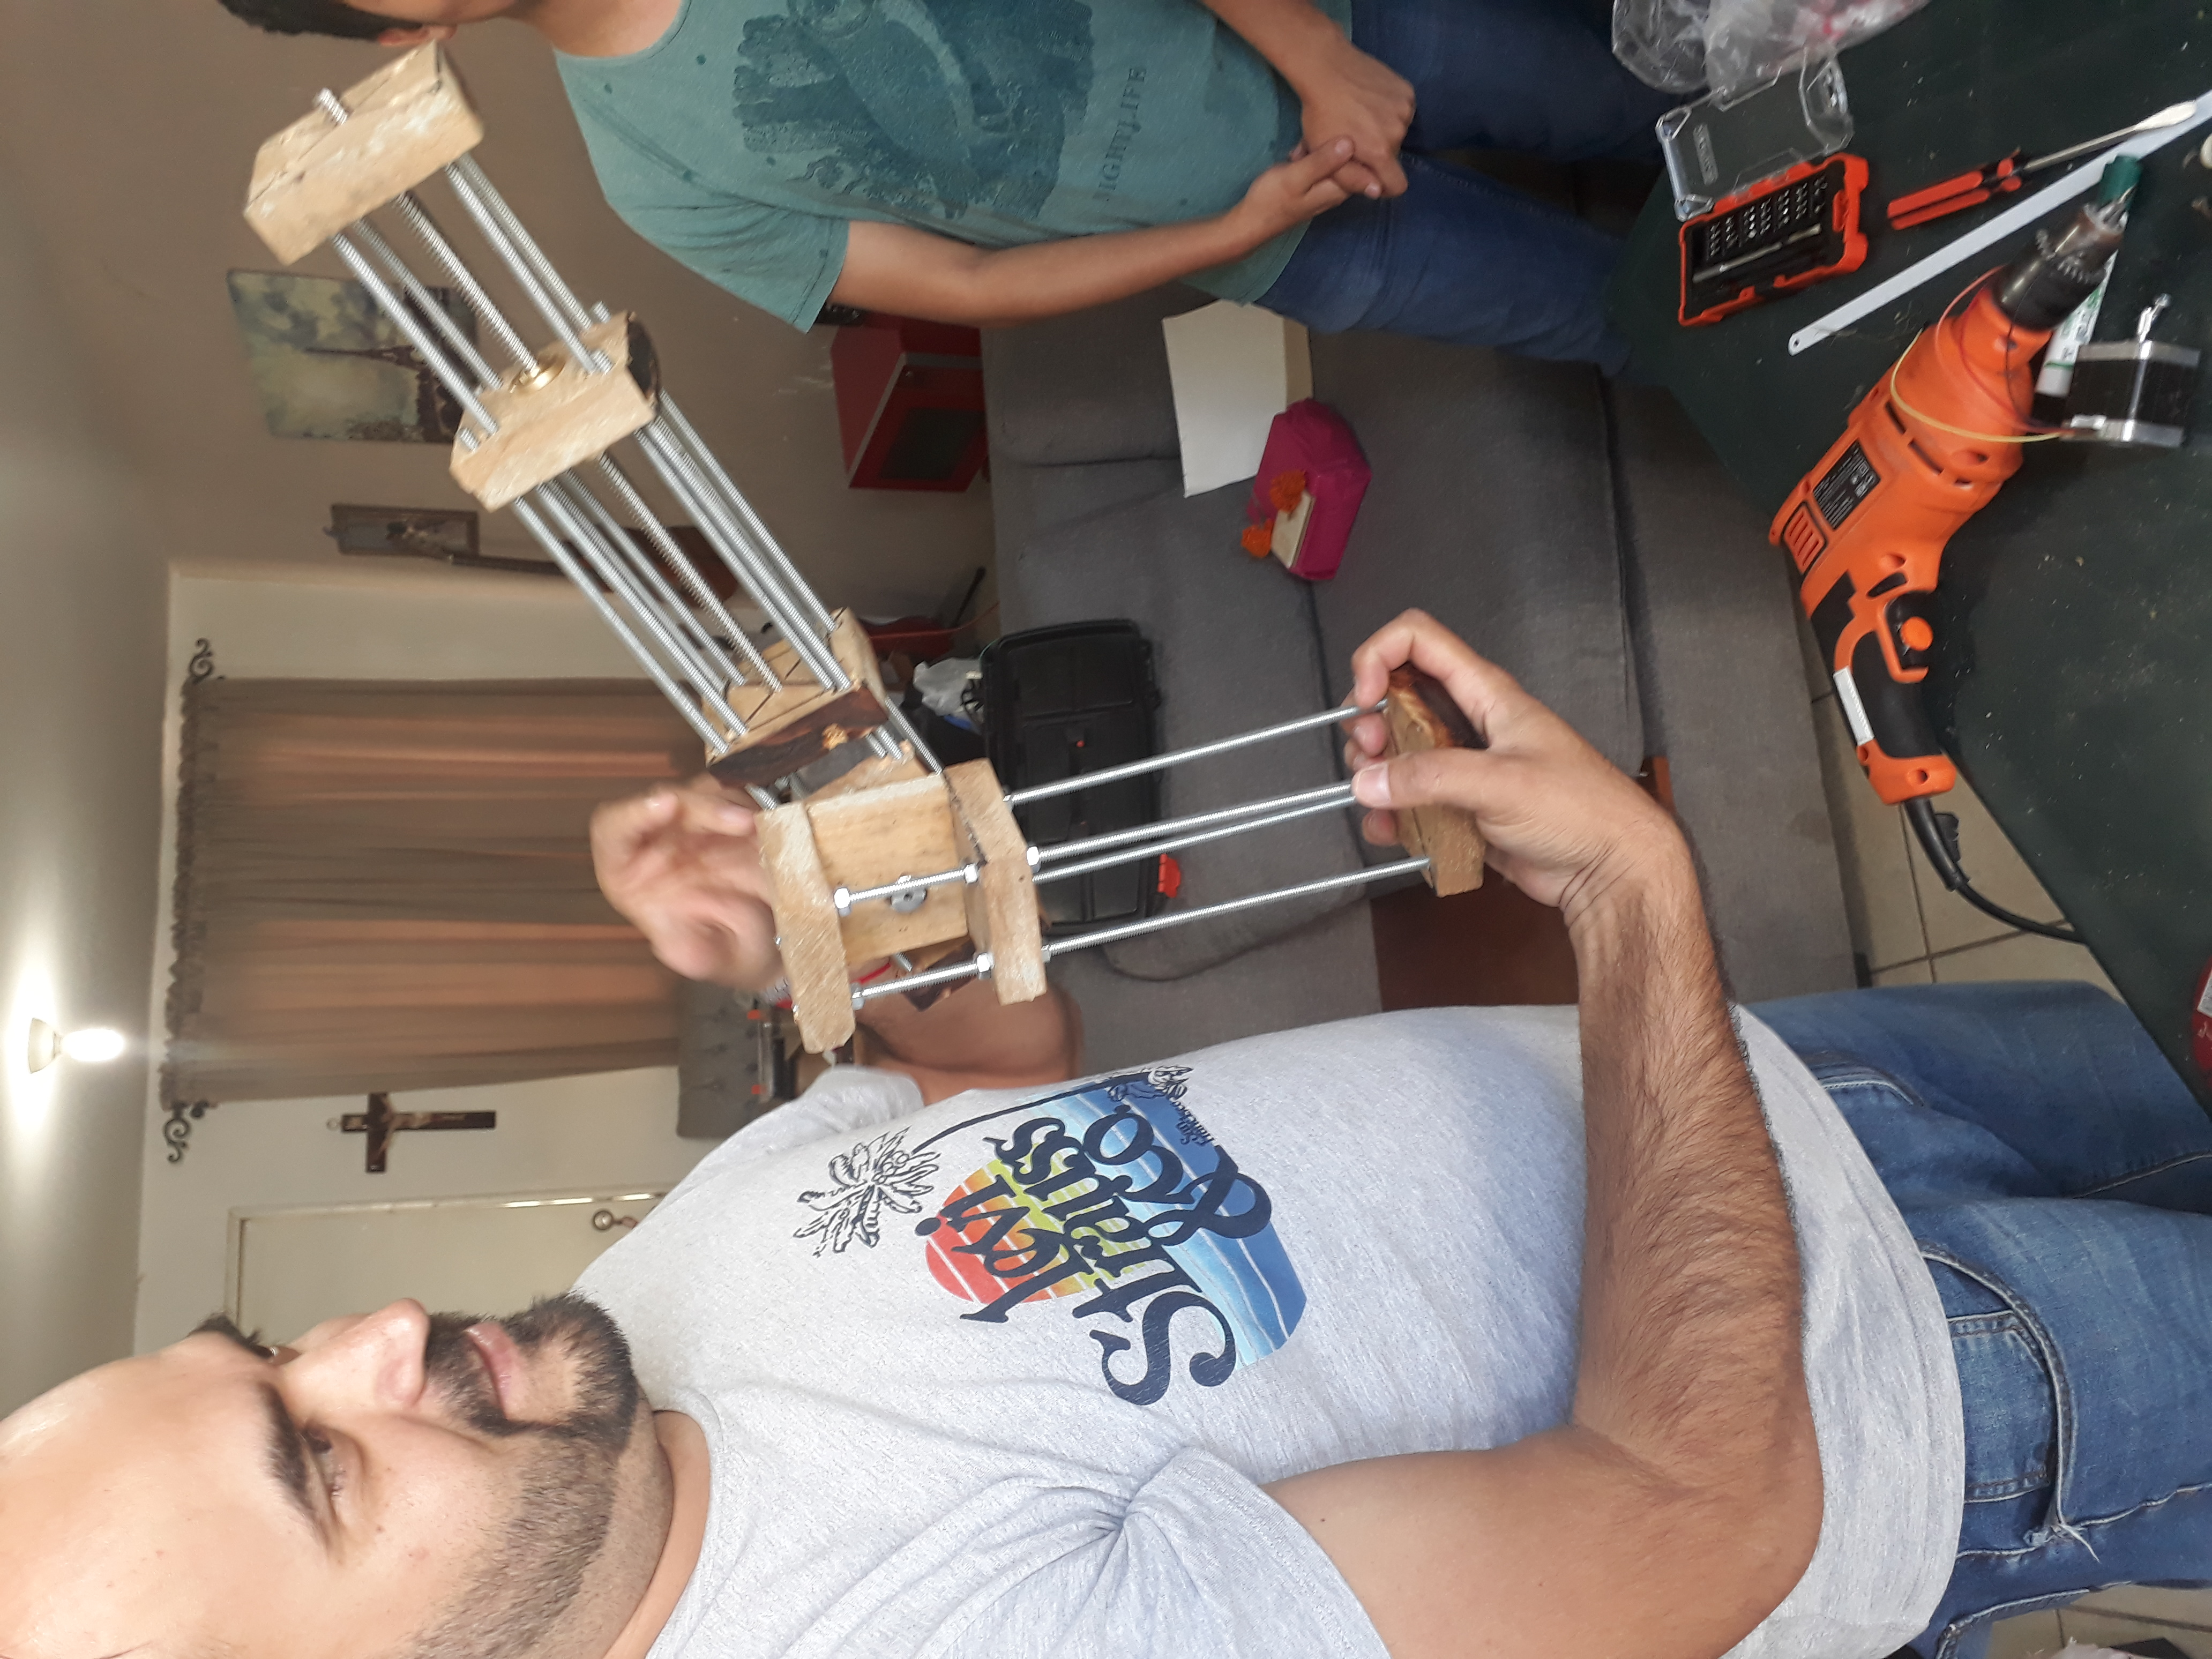
\includegraphics[scale=0.05]{9.jpg} 
\end{center}

\chapter{Conclusiones}
\section{César Alvarado}
Al realizar el proyecto en conjunto se puede demostrar que el enfoque dado para su diseño y analisis, aprendido en el curso de este cuatrimestre fue óptimo para su elaboración el cuál es arduo con algunos inconvenientes no vistos y planeados en el sistema de planeación por lo tanto concluyó con lo que se aprendió en este lapso cortó un trabajo realizado en conjunto con lo aprendido previamente en este periodo.
\section{Jonathan Fonseca}
Este proyecto nos hizo aplicar todos los conocimientos obtenidos hasta la fecha, ya que este proyecto lleva de todo; programación, diseño 3D mediante software, modelos matemáticos, etc. Aún estando sin terminar, este proyecto es la culminación de nuestra carrera, ya que también será nuestro proyecto de despedida en esta escuela.
\section{Marcos Manzo}
El haber realizado un robot desde cero, nos lleva a la conclusión sobre la importancia de realizar el estudio de un elemento antes de comenzar a trabajar con él.\\
El poder desarrollar un prototipo, con características específicas pero comenzando desde cero, nos muestra la importancia del por qué de las cosas, como una idea nos lleva a otra idea y al final del día se forma una sola pero con raíces más profundas y siempre teniendo claro el objetivo de lo que buscamos.\\
Cuesta trabajo creer, cómo fue que comenzamos a realizar el prototipo en un simple boceto, desarrollamos el análisis y hoy que tenemos un prototipo nos demuestra la importancia de todo lo que antes llevamos a cabo. Nos muestra cómo es que, con un estudio realizado incorrectamente, todo lo desarrollado no llega a cumplir los objetivos propuestos.\\
Aunque fue nuestro primer prototipo, el aprendizaje se encuentra ahí, el saber qué puntos debemos de volver a realizar y qué puntos se mantienen firmes, ya que aprender de los errores es avanzar hacia adelante
\section{Eduardo Robles}
Nuestro proyecto anual en esta primera prueba cuatrimestral ha sido desde mi perspectiva un gran avance ya que se ha puesto en el todo lo aprendido en este cuatrimestre desde el método de Denavit-Hartenberg hasta como realizar el análisis de elementos finitos.  Sin duda alguna nos encontramos con varios obstáculos como lo fue en su momento la interpretación del análisis de los elementos finitos o el armado del prototipo, pero a pesar creo que todo el equipo esta conforme con el resultado y solo esperamos mejorar el proyecto teniendo en cuenta todos los errores que cometimos para no volver a cruzarnos con ellos.
\section{Víctor Tapia}
Con este proyecto hemos puesto en práctica los conocimientos que hemos adquirido no solamente en este cuatrimestre, sino también de los pasados. Fue un completo desafío y, aunque no está del todo finalizado, es un orgullo el resultado en nuestro equipo, ver como este proyecto pasó de ser un bosquejo en una hoja reciclada a ser un elemento real.
\bibliographystyle{plain}
\cite{Morales:2009}
\cite{de2006robotica}
\bibliography{bibliografia}


\end{document}

